\documentclass[11pt]{report}
% PACKAGES
  \usepackage[a4paper,left=28mm,right=28mm,top=30mm,bottom=30mm]{geometry}
  \usepackage{graphicx,epstopdf}      % Used to import external graphics (figures)
  \usepackage{hyperref}       % Used for referring to links inside and outside the document
  \usepackage[table]{xcolor}  % To include colors 
  \usepackage{amsmath}        % For most of the math symbols and environments (such as \begin{align})
  \usepackage{amssymb}        % For using symbols in the document
  \usepackage{float}          % Arranging of figures on the page
  \usepackage[bf]{caption}    % Arranging the captions in floating environments [bf] makes the Figures bold
  \usepackage{subcaption}     % To arrange captions of subfigures
  \usepackage{booktabs}       % For standard tabular tables, with rules
  \usepackage{tabularx}       % For clean tables such as in the Nomenclature
  \usepackage{fancyhdr}       % Fancy headers
  \usepackage[colorinlistoftodos]{todonotes}      % To create todo notes
  \usepackage[nottoc,notlot,notlof]{tocbibind}    % Add bibliography to content
  \usepackage{bm}             % Make bold symbols
  \usepackage{lipsum}
  \usepackage{parskip}
% LAY-OUT
  % \usepackage{pdfpages}

  % \usepackage{pdflscape}

   \renewcommand\thesection{\arabic{section}}

  % \usepackage[mathletters]{ucs}
  % \usepackage[utf8x]{inputenc}
  %Bibliography for references, with reference style options
  \usepackage[
  backend=biber,
  bibstyle=ieee,
  citestyle=numeric-comp,
  dashed=false,
  url = false,
  maxnames=8,
  maxcitenames=2,
  mincitenames=1,
  sorting=none,
  isbn = false,
  doi = false
  ]{biblatex}
  \addbibresource{references.bib}

  %Set the page style
  \pagestyle{fancy}
  \fancyhead[L]{\ifodd\value{page} \slshape\nouppercase{\rightmark} \else \fi}
  \fancyhead[R]{\ifodd\value{page} \else \slshape\nouppercase{\leftmark} \fi}
  \chead{ }
  \lfoot{}
  \rfoot{}
  \cfoot{\small\thepage}


  %Give colors to links/refs etc
  \hypersetup{colorlinks, linkcolor={blue!0!black}, 
                          citecolor={blue!70!black}, 
                           urlcolor={blue!80!}} 
                       
  %% Set up numbering and spacing
  \numberwithin{equation}{section}        %Number the equations per section
  \numberwithin{figure}{section}          %Number the figures per section
  \numberwithin{table}{section}           %Number the tables per section
  \captionsetup[table]{skip=1pt}          %Skip 1 pt after a table
  \captionsetup[figure]{skip=3.5pt}       %Skip 4 pt after a figure
  \setcounter{secnumdepth}{3}             %Count up to the subsubsection 
  \setcounter{topnumber}{1}               %Number of floats at top of a page (default is 2)

  %%%%% proof/theorem/definition boxes

  \usepackage{cleveref}
  \usepackage[most]{tcolorbox}
  \newtcbtheorem{Theorem}{Theorem}{
    enhanced,
    sharp corners,
    attach boxed title to top left={
      yshifttext=-1mm
    },
    colback=white,
    colframe=blue!75!black,
    fonttitle=\bfseries,
    boxed title style={
      sharp corners,
      size=small,
      colback=blue!75!black,
      colframe=blue!75!black,
    } 
  }{thm}

  \newtcbtheorem{Definition}{Definition}{
    enhanced,
    sharp corners,
    attach boxed title to top left={
      yshifttext=-1mm
    },
    colback=white,
    colframe=blue!25,
    fonttitle=\bfseries,
    coltitle=black,
    boxed title style={
      sharp corners,
      size=small,
      colback=blue!25,
      colframe=blue!25,
    } 
  }{def}

  \newtcbtheorem[no counter]{Proof}{Proof}{
    enhanced,
    sharp corners,
    attach boxed title to top left={
      yshifttext=-1mm
    },
    colback=white,
    colframe=blue!25,
    fonttitle=\bfseries,
    coltitle=black,
    boxed title style={
      sharp corners,
      size=small,
      colback=blue!25,
      colframe=blue!25,
    } 
  }{prf}
% DEFINITIONS
  %% Titlepage definitions
  \newcommand{\deltitle}{Impact-Aware Control for a Dual-Arm Setup}      %Your project title
  \newcommand{\StudentName}{Gijs van den Brandt}  %Student name
  \newcommand{\StudentID}{1257110}                    %Your student number
  % \newcommand{\DCcode}{2021.109}                      %Get your DC code from the D&C secretariat

  %% Operators
  \DeclareMathOperator\sign{sgn}                      %Sign function
  \DeclareMathOperator\diag{diag}                     %Diagonal operator
  \DeclareMathOperator\imag{Imag}                     %Imaginary part of complex variable
  \DeclareMathOperator\real{Real}                     %Real part of complex variable
  \DeclareMathOperator*{\argmin}{\arg\!\min}          %Argmin operator
  \newcommand{\norm}[1]{\left\lVert#1\right\rVert}    %Norm operator

  %% Variable definition
  \newcommand{\R}{\mathbb{R}}                         % Set of real numbers
  \newcommand{\C}{\mathbb{C}}                         % Set of complex numbers

\begin{document}

% Summary 
  \section*{Progress meeting 9 | 7 October, 2022}


  \section*{1. Progress}
  \begin{itemize}
  \item \textbf{Teleoperation:} 
    
  \item \textbf{Custom end effector:} 
    
  \item \textbf{Impact detection:} 

  \item \textbf{Learning from demonstration:} 
    
  \end{itemize}

  \section*{2. Agenda}
  During the meeting, I would like to discuss the following points:

  \begin{itemize}
      \item  
      \item 
  \end{itemize}

  \section*{3. Next steps}

  \begin{itemize}
      \item  
      \item 
  \end{itemize}

  \section*{4. Long-term planning}
  Below is the current long-term planning for the project phase. The description of the labeled subjects are given in the preparation phase report and are also provided on the next page.

  \begin{figure}[H]
  \centering
  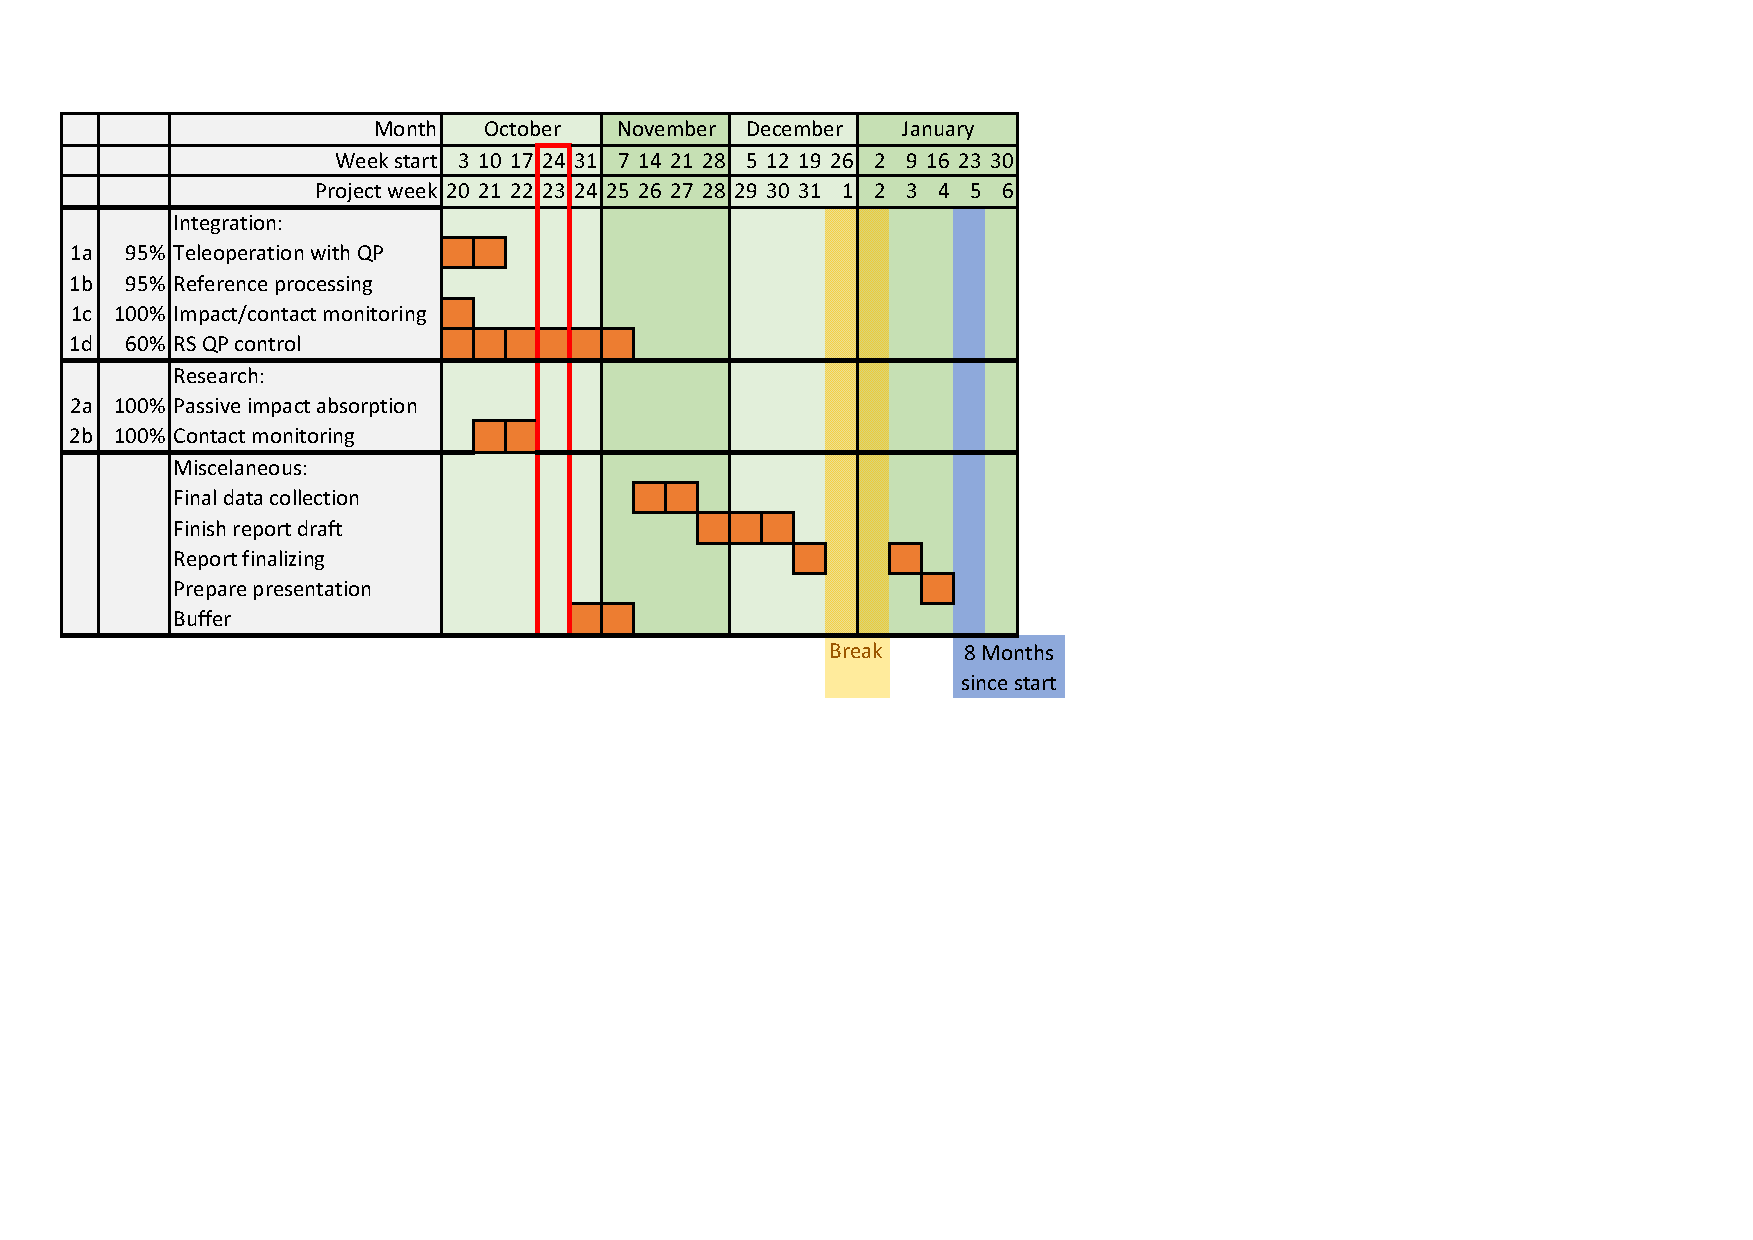
\includegraphics[width=0.7\textwidth, trim={0.87cm 9.5cm 10cm 1.5cm},clip]{graphics/planning v2.pdf}

  \label{fig:my_label}
  \end{figure}

  \begin{enumerate}
  \item[1a] \textbf{Translating dual-arm teleoperation to the physical setup.} The existing implementation in simulation already uses the mc\_rtc interface, meaning that the switch to reality shouldn't pose an issue. Nevertheless, this step also involves getting familiar with the software, which increases the anticipated time for this step.
  \item[1b] \textbf{Extracting references from the demonstration data.} The demonstrated trajectories should be split into ante-impact and post-impact sections, and extended to facilitate RS. Furthermore multiple measurements should be used to fit ProMPs, after which a reference can be generated. It is also key to identify which data should be learned from the demonstration. This is not limited to choosing between a force or position reference, but can also consists of learning properties of the environment, e.g. friction cones or box inertia, that are crucial to a dual-arm box grabbing scenario.
  \item[1c] \textbf{Integrating impact detection and contact monitoring in mc\_rtc.} The majority of the impact detector's complexity resides in the momentum observer; however, Franka Emika's software already has an integrated momentum observer. This still leaves tuning of the impact detecting algorithms which might be time consuming. Furthermore an analysis comparing the available methods could be worthwhile. Factors which determines the effectivity of the impact detection algorithm include speed of detection, as well as reliability, i.e. the rate of false positives. The addition of objects that cause unexpected impacts is not considered a part of the research scope.
  \item[1d] \textbf{Configuring QP controllers for the ante-impact, intermediate, and post-impact phase.} For each of the phases, it is important to address the redundancy in the arms' degrees of freedom. After that, control for the ante-impact phase should be trivial. For the intermediate phase, it is expected that ante-impact reference tracking without velocity feedback should be applicable on a dual-arm robot, though this might prove to be false, in which case other methods should be investigated. During post-impact control, the challenge will be maintaining non-slip contact with the box. It is difficult to say how well the results from simulations can be repeated with torque control, where the state of the box can not be sensed to be used in the QP controller.
   \item[2a] \textbf{Passive impact absorption:} A soft cover for the end effector will be designed. Such a cover can be connected to the Panda by connecting bolts to the so-called flange interface. A mold will be created using 3D printing to allow for casting of various silicone soft covers. Design parameters -- i.e. material properties (controlled by choosing different kinds of silicone) and soft cover thickness -- will be analyzed experimentally. A systematic comparison between various designs will require an experiment plan including a realistic testing scenario. Evaluation of performance can be based on the oscillatory response in position and force after establishing contact. Furthermore multiple scenarios with various box surface properties and robot poses should be considered.
  
  \item[2b] \textbf{Contact monitoring:} When investigating contact monitoring, two approaches can be taken: either using proprioceptive or exteroceptive sensors. A possible improvement for contact monitoring using proprioceptive sensors could be to wait a fixed time starting from the last detected impact, rather than waiting a fixed time from the first impact. As for exteroceptive sensors, they can be a hurdle for large-scale commercial applications as they are not integrated in the robot. However, if a soft cover is to be mounted to the end effector, including tactile sensors for impact and contact monitoring becomes more feasible. Practical questions such as which tactile sensor to use and how to integrate it could be addressed, though this is not absolutely necessary for completing the research goals, and therefore has a low priority.
  \end{enumerate}
% main text
  \newpage
  \section{Impact detection using contact force vs velocity}
  For impact detection, Benn and Sven considered two options: looking at jumps in velocity, or jumps in force. Ultimately, Benn and Sven both ended up using the forces, whereas I think looking at velocities makes more sense in the context of reference spreading. This section explains my reasoning.

  Looking at jumps in force for impact detection could result in false positives. Consider an end effector that is already exerting a contact force on a fixed surface using impedance control. A jump in the reference would result in a jump in the contact force. Even if contact is maintained throughout the event, the jump in contact force would trigger the impact monitor while no impact has actually occurred. In the described situation, the velocity remains unchanged, meaning that a velocity-based impact detector would not return a false positive.

  Additionally, contact forces cannot be directly measured, and the process of estimating them with a momentum observer is quite complex and involves a delay when compared to determining the velocity. 

  Given the downsides of looking at force rather than velocity, there must be significant benefits to warrant using force estimates for impact detection. I am not able to fully identify Benn's reasoning here (he states that "The most common method of impact detection is through the use of external joint torque estimators", though I suspect this is in the context of human safety). Sven, however, does provide an argument. In his experiments, he noticed that velocity data was missing during some timesteps, which resulted in poor impact detection. The impact detector using force did not suffer from this issue.

  As discussed during the questions of Sven's defense, the momentum observer acted as a filter which made it so that missing data was not problematic for the impact detector that uses force. Therefore I don't think that missing velocity data is a valid argument for looking at force data; applying a filter to account for missing velocity data makes more sense in my opinion.

  As a final argument, the reason for applying reference spreading is diminishing peaks in the velocity tracking error. If a jump in velocity cannot be measured, then it is also not possible for the velocity tracking error to peak (barring a peak in the reference). While there is some connection between the peaking error and contact forces, the connection between measured velocity and the peaking error is much closer.
  
  \newpage

  \section{Learning impedance vs force/position reference}
  When considering what reference to extract from demonstrations, two options come to mind. Firstly, it is possible to look at the position trajectory of the robot during demonstration. As the robot position by itself does not fully describe the robot's state, a force reference should also be extracted. This resembles the approach used by Sven. A second option would be to learn an impedance reference, i.e., the position of the VR device, which encapsulates both position and force. This section describes how both approaches would be implemented, as well as listing the pros and cons. 

  As a disclaimer, it should be noted that neither Sven's implementation nor the current VR implementation utilize a velocity reference. While Sven used reference spreading for the force reference, the value of reference spreading might be more apparent when applied to a velocity reference. The tracking performance is also expected to improve with the addition of a velocity reference. Therefore, the remainder of this section will assume that a velocity reference is included in the control scheme. Obtaining this reference should not prove difficult as a robot's velocity can easily be determined, and the HTC Vive provides velocity (and even acceleration) measurements.

  \subsection{Impedance reference}
  - 

% BIBLIOGRAPHY

  \newpage
  \addcontentsline{toc}{chapter}{References}
  \printbibliography[title=References]

  \newpage
  \thispagestyle{empty} \ \newpage


\end{document}